% ------------------------------------------------------
\chapter{Tesztelési eredmények}
% ------------------------------------------------------

Az alábbi mérési eredményeket ugyanazon tesztpéldákon végeztem el mindhárom módszerre. A használt videókártya egy Nvidia GTX 1060 Ti notebook GPU. A felbontás minden esetben Full HD.

\begin{figure}[H]
	\centering
	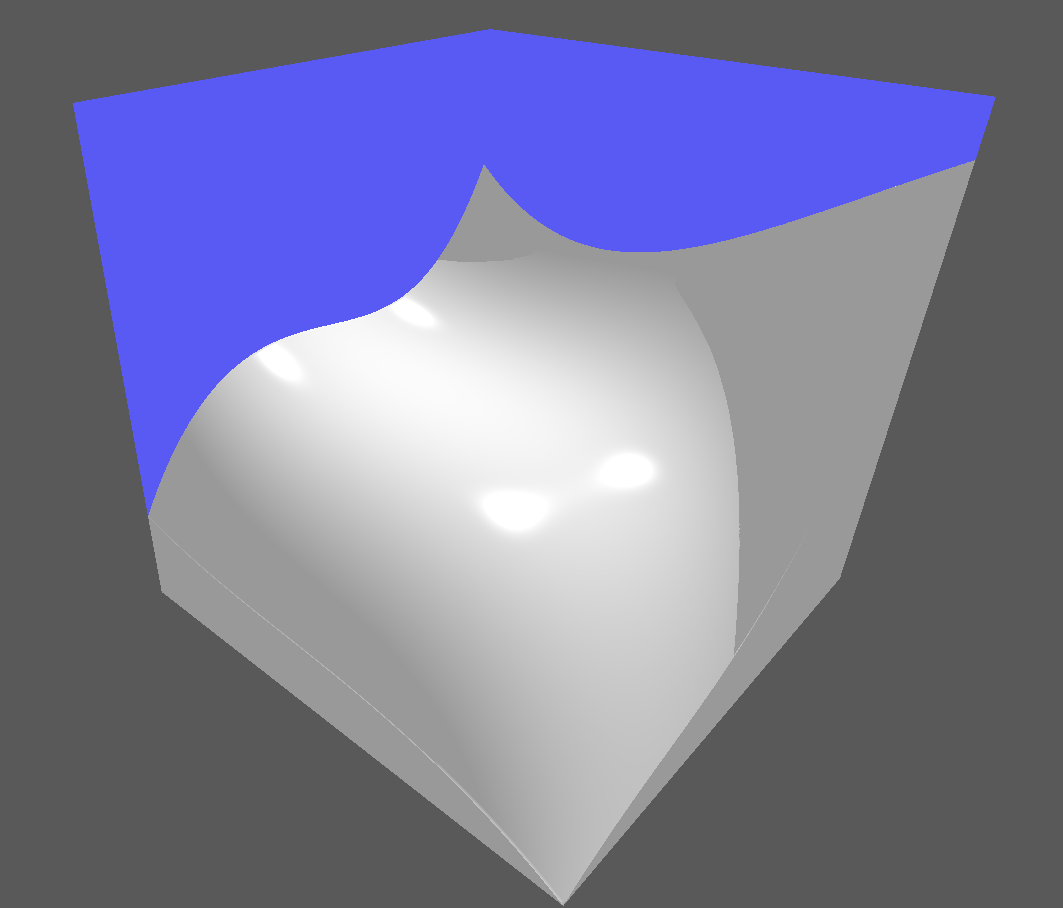
\includegraphics[width=0.5\textwidth]{result.png}
	\caption{Bézier-felület}
	\label{img:bezSurf}
\end{figure}

\section{Generálási módszer hatása a sugárkövetésre}

Itt azt hasonlítom össze, hogyan hat a sphere trace algoritmus futási idejére a generálási módszer. \Aref{tab:trace} táblázat utolsó oszlopa 512 képkocka megjelenítésének átlagos GPU-idejét foglalja össze. A jelenetben minden esetben egy véletlenszerűen generált Bézier-felület és egy pontfényforrás szerepelt, amihez ún. kemény árnyékokat számítottam.

\begin{table}[H]
	\begin{center}
		\begin{tabular}{| c || c | c |}
			\hline
			\textbf{Generálási módszer} & \textbf{Szükséges lépésszám} & \textbf{Átlagos GPU idő (ms)} \\ 
			\hline\hline
			Lipschitz & $512<$ & 1,47 \\
			\hline
			Brute force & $<256$ & 0,95 \\
			\hline
			Adam & $<256$ & 0,96 \\
			\hline
		\end{tabular}
	\end{center}
	\caption{Generálási módszer hatása a sugárkövetésre}
	\label{tab:trace}
\end{table}

\subsection{Lipschitz-módszer}
A Lipschitz-módszer időköltsége a memóriaigénnyel egyenesen arányos. Az ilyen algoritmusok minden esetben memórialimitáltak. A generált távolságmező olyan rossz minőségű, hogy alacsony látószögből még 512 lépésben sem konvergál a sugárkövetés. A generálás emellett olyan olcsó, hogy akár sugárkövetéskor, a pixel shaderben is kiszámítható. Ezt a módszert a következőkben nem tárgyalom.

\subsection{Brute Force módszer}
A Brute Force módszer meglehetősen költséges, azonban a generált távolságmező (a rácspontokban) biztosan optimális, így 256 iteráció minden esetben elég volt.

\subsection{AdaMax módszer}
A tesztek meglepő eredménye, hogy az AdaMax algoritmusban 25-nél nagyobb iterációszám egy esetben sem javított a képminőségen. Ennek egyik oka, hogy a felület közelében a 10. pont miatt nagyon gyorsan konvergál a módszer. Másik oka, hogy ha a sugárkövetés során beleszaladunk a felületbe egy rossz becslés miatt, akkor a következő távolságkiértékelés negatív lesz, és visszatalálunk a felülethez. A sugárkövetéshez továbbra is elegendő volt 256 iteráció minden esetben, így kijelenthetjük, hogy a szimulációs eredményeket sikerült megerősíteni.


\section{Távolságmező-generálás}
Mivel a Lipschitz-módszer csak egy gyenge alsó közelítést ad a távolságmezőre, így a Brute Force algoritmust hasonlítottam össze az AdaMax algoritmust használó  módszerrel. \Aref{tab:gen} táblázatban az előbb bemutatott tesztpélda távolságmezőjének generálásához szükséges átlagos GPU-idők szerepelnek a felbontás függvényében, milliszekundumban.

\begin{table}[H]
	\begin{center}
		\begin{tabular}{| c || c | c | c | c | c | c | c | c |}
			\hline
			\textbf{Felbontás} & 16	& 32 & 48 & 64 & 80 & 96 & 112 & 128 \\ 
			\hline\hline
			\textbf{Brute force} & 0.17 & 2.18 & 16.87 & 52.23 & 185.79 & 382.57 & - & - \\
			\hline
			\textbf{AdaMax} & 1.09 & 4.36 & 15.82 & 28.04 & 63.49 & 92.65 & 163.07 & 219.13
			\\
			\hline
		\end{tabular}
	\end{center}
	\caption{A generálás ideje a felbontás függvényében, milliszekundumban}
	\label{tab:gen}
\end{table}

Az értékeket \aref{img:bf-adam} grafikonon meg is jelenítettem:

\begin{figure}[H]
	\centering
	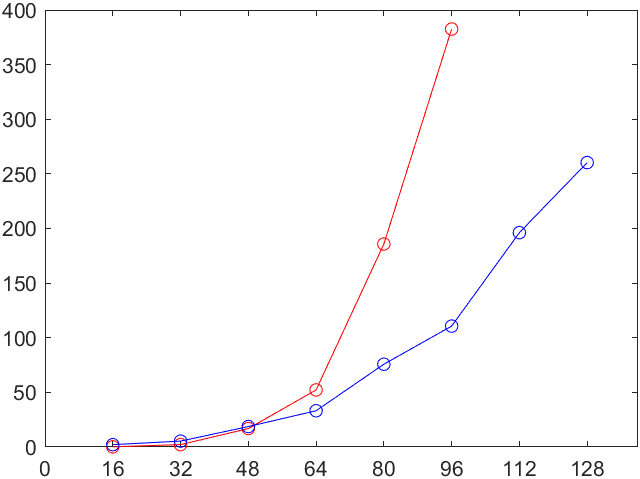
\includegraphics[width=0.4\textwidth]{bf-adam.png}
	\caption{A generálás ideje a felbontás függvényében, milliszekundumban}
	\label{img:bf-adam}
\end{figure}

\Aref{tab:gen} teszt eredményeiből látszik, hogy a két módszer algoritmikus komplexitásából adódó különbségek már kis felbontás esetén ($64^3$) is jelentősek. A komplexitásbeli különbség oka, hogy amíg a Brute Force megoldás a függvényt egyre növekvő felbontáson értékeli ki, addig az új módszer fix lépést végez 10 pontból.

\section{Összehasonlítás a tesszellációval}
A felületet a sugárkövetés mellett háromszögekkel közelítve is megjeleníthetjük. A két módszer eltéréseit úgy tudjuk vizualizálni, ha sugárkövetés után a fragment shaderben beleírjuk a mélység adatot a mélység bufferbe, és az egyik felület árnyalását valami egyszerűre cseréljük. \Aref{img:zfight} ábrán  a sugárkövetett felületet Blinn--Phong-árnyalással, a háromszögekkel tesszelláltat pedig egy egyszerű színskálával jelenítettem meg.

\begin{figure}[H]
	\centering
	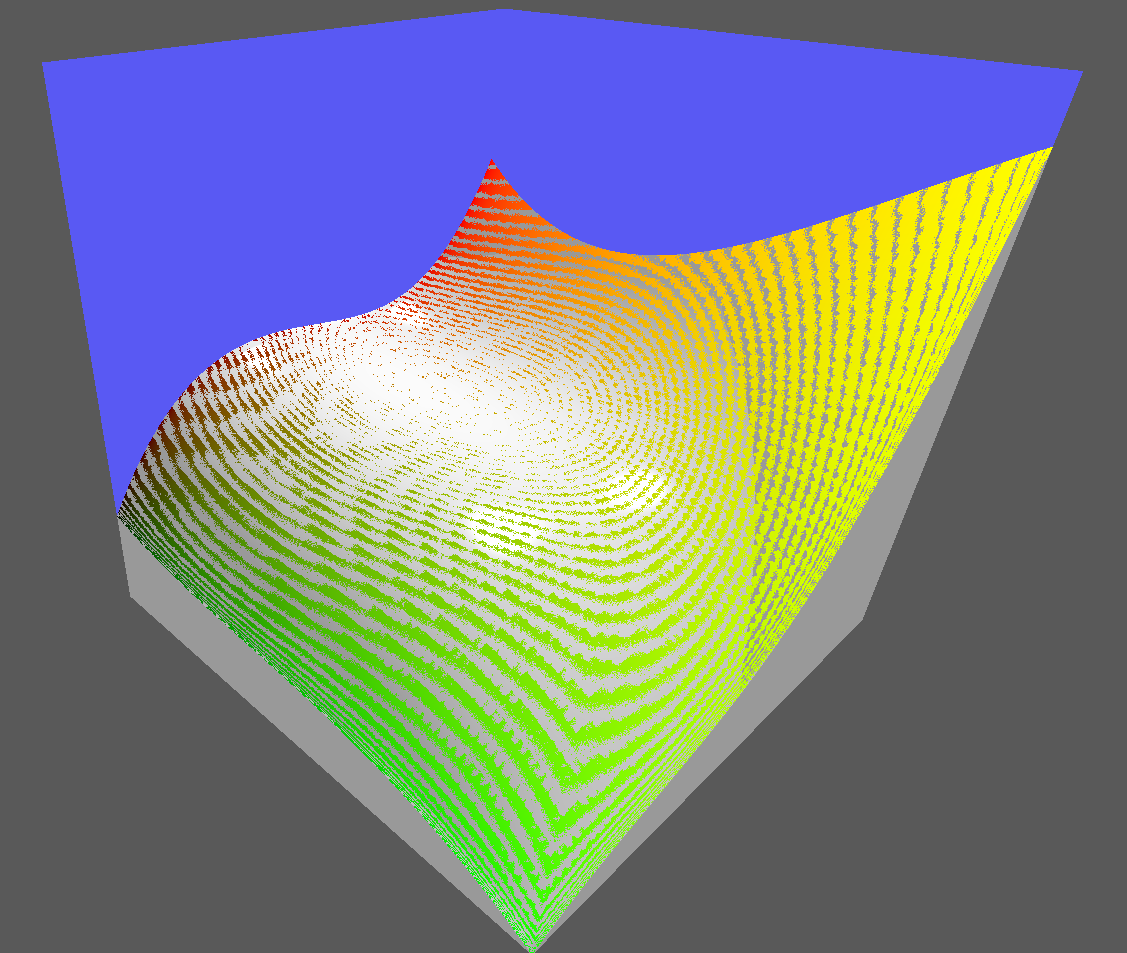
\includegraphics[width=0.4\textwidth]{zfight.png}
	\caption{Tesszellált és sugárkövetett felület egyszerre kirajzolva}
	\label{img:zfight}
\end{figure}

\Aref{img:zfight} ábrán a két módszerrel kirajzolt felület színe váltakozva jelenik meg. Ennek oka, hogyha a mélységbuffer értékei helyesek, akkor átlátszatlan felületeknél minden pixel színe a legközelebbi felület színe lesz. A váltakozás oka, hogy amíg felületet tartalmazó voxelekben a sugárkövetés egy bilineáris felületet határoz meg, addig a raszterizációnál a felületet két, a csúcspontokban interpoláló háromszöggel közelítjük.

A raszterizációt felhasználhatjuk arra, hogy az első sugárkövetést megspóroljuk és csak az árnyékokhoz használjunk sugárkövetést. Ezt a technikát használják például az Unreal Engine-ben is puha árnyékok számításásra. \cite{RayTracedDistanceFieldShadowing} \Aref{tab:rast} táblázatban egy, az előzőektől független teszt eredményei láthatók. A második oszlopba egy képkocka kirajzolásához szükséges átlagos GPU-idő került.

\begin{table}[H]
	\begin{center}
		\begin{tabular}{| c || c | c |}
			\hline
			\textbf{Generálási módszer} & \textbf{Átlagos GPU idő (ms)} \\ 
			\hline\hline
			Lipschitz & 0,72 \\
			\hline
			Brute force & 0,51 \\
			\hline
			AdaMax & 0,50 \\
			\hline
			Háromszögelés + AdaMax & 0,24 \\
			\hline
		\end{tabular}
	\end{center}
	\caption{Sugárkövetés helyettesítése raszterizációval}
	\label{tab:rast}
\end{table}





% ------------------------------------------------------
\chapter{Összefoglalás}
\label{ch:sum}
% ------------------------------------------------------

A dolgozatomban bemutattam és implementáltam a távolságmezők generálásának alapvető módszereit, majd áttekintettem a parametrikus- és Bézier-felületek elméleti hátterét. Fő eredményként bemutattam, hogyan használhatók gradiens módszerek távolságmezők generálásához, és szimulációval validáltam az AdaMax algoritmus alkalmazhatóságát köbös Bézier felületek távolságmezőjének generálására. Kitértem a módszer GPU-implementációjának részleteire, mellyel nagyságrendekkel gyorsítottam a kiértékelést. Végül mérésekkel igazoltam, hogy az új módszer már kis felbontáson is lényegesen gyorsabb, mint a referencia implementáció.
